% ===================== 担当D =====================
\section{担当D — 音響合成（Processing/Minim）}

\subsection{部品一覧}

本システムで使用する主な部品を以下に示す．
本担当は5パート分のユニットを構成するため，以下の部品を各5台用意する．

\begin{table}[h]
  \centering
  \caption{担当D 部品一覧}
  \label{tab:parts_d}
  \begin{tabular}{llrl}
    \hline
    部品名 & 型番・仕様 & 数量 & 用途 \\
    \hline
    PC（Processing実行環境） & Processing 4.x + Minim対応 & 5 & 音響合成・音声出力 \\
    スピーカーまたはヘッドフォン & — & 5 & 音声再生 \\
    USB Type-Cケーブル & — & 5 & Arduino子機との接続 \\
    \hline
  \end{tabular}
\end{table}

\subsection{ハードウェア設計}
本担当では，PC上での音響処理を主体とするため，専用の電子回路は使用しない．
Arduino子機（担当C）からUSB Type-C Serialを介してデータを受信し，
PC上のProcessing/Minimにより音響合成を行い，スピーカーへ音声出力する．

本担当は5パート分のユニットを独立して構成し，
各ユニットはArduino子機1台・PC1台・スピーカー1台の組で動作する．

なお，各PCはArduino子機1台と1対1でUSB接続されるため，
受信した4バイトパケットはそのPCが担当するパートの音響合成のみに使用する．

\begin{figure}[H]
  \centering
  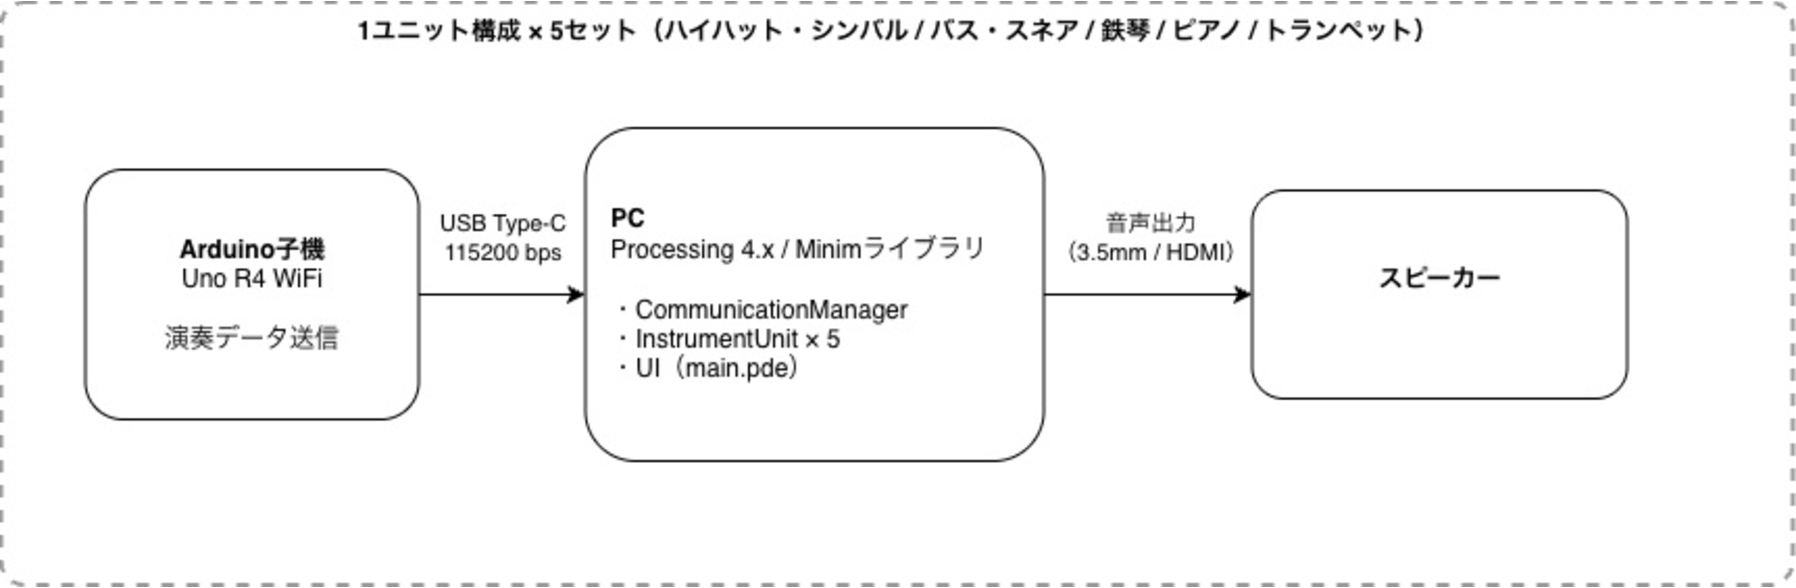
\includegraphics[width=0.85\linewidth]{figures/tantoD/hardware_connection_diagram_D.pdf}
  \caption{ハードウェア接続図（1ユニット構成 × 5セット）}
  \label{fig:hardware_D}
\end{figure}

115200\,bpsのUSBシリアル通信で4バイトパケット（NOTE\_OFF / NOTE / VEL / LONG）を受信する．

\subsection{楽器音色設計の方針}

聴衆が音楽として自然に認識できるよう，音響工学的な知見に基づき，
各ユニットに明確な役割を持たせた音色設計を行う．

\subsubsection*{楽器グループの役割}
\begin{itemize}
  \item ピアノ・鉄琴・トランペット（主旋律担当）\\
  倍音成分を調整し，メロディの明瞭さを追求する．
  基本振幅を高く設定し，常に聴衆の注意を引く音圧とする
  （基準音量1.0に対し0.8〜1.0）．

  \item バス・スネア（リズムの土台）\\
  低域のエネルギーとアタックの鋭さで拍を明示する．
  主旋律を埋もれさせない範囲で，演奏の骨格を維持するために
  十分な音圧を確保する（基準音量1.0に対し0.6〜0.7）．

  \item ハイハット・シンバル（リズムのアクセント）\\
  高域の金属音で演奏の華やかさを強調する．
  リズム楽器と同様の音量方針とする（基準音量1.0に対し0.6〜0.7）．
\end{itemize}

\subsubsection*{音色設計のアプローチ}
楽器の音色をデジタル環境で再現するにあたり，以下のプロセスに基づいた設計を行う．

\begin{enumerate}
  \item 物理特性分析：対象楽器の周波数成分を調和倍音の重なり
  （ピアノ・鉄琴・トランペット）と非調和・ノイズ成分（打楽器）に分類する．

  \item 合成手法選定：加算合成による倍音構築か，
  ホワイトノイズをベースとした減算合成か，
  目的の音響モデルに応じて決定する．

  \item 質感調整：ADSRエンベロープによる時間変化と，
  LowPass / BitCrusherによる高域・ビット深度の制御を行い，
  聴覚的な違和感を排除する．
\end{enumerate}

各パラメータの妥当性確認にあたっては，外部ツールを用いて既存音源と生成音の
スペクトラムを比較し，基音および主要倍音の構成を確認しながら
ADSRパラメータおよびフィルタ設定を逐次調整する．


\subsection{音楽的表現の設計}

指揮者のリアルタイムな動作に応じた変化が，
人間らしい演奏として知覚されるための制御方針を以下に定める．

\subsubsection*{フェルマータの自然な表現}
通信仕様をNOTE\_OFFフラグ付きパケット方式としたことで，
フェルマータの表現がより自然なものとなった．
指揮者が静止した際，担当Cが次パケットの送信を保留することで，
Processing側は特別な処理を行わずともADSRのSustain状態が自動的に延長される．
これにより，デジタル処理の不自然さを感じさせない，
生身の演奏に近い「溜め」を実現する．

演奏再開時は，腕再開後に担当Cから次パケット（NOTE\_OFF=1）が送信されることを
トリガーとしてReleaseを開始し，前の音の余韻を次音に滑らかに溶け込ませることで，
デジタル特有の不自然な音切れを回避する．

\subsubsection*{テンポ変化時の自然な追従}
テンポ変化に対し，デジタル的な違和感を排除するための配慮を組み込む．
急なテンポアップ時に前の音が残っていても，消音せずに新しい音を重ねる
多重発音を許容し，残響が途切れる不自然さを解消する（NOTE\_OFF=0時の動作）．
またテンポ加速時はRelease時間を短縮して歯切れを良くし，
減速時はReleaseを延長して空白を響きで埋めることで，
どの速度域でも自然な響きを維持する．


\subsection{楽器別音響パラメータ}

各楽器のADSR設定，倍音比率，および適用するエフェクトの数値を
表\,\ref{tab:adsr_params}に示す．
なお，表中のDecay・Release値は基準（4分音符相当）の値であり，
実装ではLONG（音価）に応じた倍率を乗じて響き・余韻の長さを調整する
（2分音符は長め，8分音符は短め）．
実装段階においては，アンサンブル全体のバランスや
指揮への追従性を考慮し，聴感上の自然さを優先して逐次微調整する方針とする．

\begin{table}[h]
  \centering
  \caption{楽器別詳細パラメータ一覧}
  \label{tab:adsr_params}
  \small
  \begin{tabular}{lp{4.5cm}cccccc}
    \hline
    楽器名 & 波形構成・倍音比率 & A {[s]} & D {[s]} & S {[lvl]} & R {[s]} & フィルタ & Bit \\
    \hline
    ピアノ
      & 9倍音（微小インハーモニシティ）＋二段減衰＋ハンマーノイズ(PINK)
      & 0.002 & 0.18／12.5 & 0 & 0.50 & 5〜10\,kHz (LP) & なし \\
    鉄琴
      & 7モード（非整数比・基音$\times$4）＋打撃ノイズ
      & 0.002 & 0.08〜1.20 & 0 & 0.85 & 14000\,Hz (LP) & 16 \\
    トランペット
      & 20倍音ウェーブテーブル＋ビブラート(5.5\,Hz)＋息ノイズ
      & 0.075 & 0.18 & 0.62 & 0.85 & 9000\,Hz (LP) & 16 \\
    バスドラム（キック）
      & body 150$\to$50\,Hz＋punch 240$\to$80\,Hz＋クリック
      & 0.001 & 0.36 & 0 & 0.10 & 4200\,Hz (LP) & 16 \\
    シンバル系
      & 非整数モード多数の加算合成（実音源STFT解析ベース）※
      & \multicolumn{6}{c}{波形生成時に内包（実効: 立上り$\approx$0.05\,s，減衰は高域ほど速く余韻長め，中心$\approx$4.8\,kHz）} \\
    \hline
  \end{tabular}
\end{table}

\noindent
※\,シンバルのみ音源を\texttt{Sampler}（事前生成したモーダル波形）とする．
波形は実音源のSTFT解析（スペクトル重心が減衰とともに約8\,kHzから約3\,kHzへ降下し，
各時刻で数百のモードをもつ特性）に基づいて生成し，アタック・減衰・スペクトル整形は
波形生成時に内包する．他楽器がOscilを音源とする点のみ異なり，
\texttt{out}への接続構造（音源UGen $\rightarrow$ 出力）は全楽器で共通である．

\vspace{0.3em}
\noindent
注\,A/D/S/R欄は主要成分の代表値である．ピアノ・鉄琴は倍音（モード）ごとに個別のADSRをもち，
ピアノは二段減衰（プロンプト約0.18\,s＋アフターサウンド約12.5\,s）でBitCrusherは不使用．
バスドラムはドラムセットのキックを対象とし，振幅・ピッチを\texttt{Line}で整形する．

\subsection{ソフトウェア設計}

\subsubsection{ファイル構成}

本システムはProcessingスケッチとして実装し，以下の構成とする．

\begin{itemize}

  \item \texttt{main.pde} \\
  システム全体の制御を行う．
  初期化（\texttt{setup()}），メインループ（\texttt{draw()}），
  およびUIコンポーネント（ポート自動接続・マスターボリューム・受信データモニタ）を含む．

  \item \texttt{CommunicationManager.pde} \\
  シリアル通信の受信および4バイトデータのパース処理を行う．
  NOTE\_OFFフラグに基づく前音消音および新規発音イベントを生成し，InstrumentUnitへ通知する．
  各PCは担当パートのInstrumentUnit1インスタンスのみに通知する．

  \item 楽器別ファイル（\texttt{piano.pde}, \texttt{tekkinn.pde}, \texttt{toranpet.pde}, \texttt{basudoramu.pde}, \texttt{sinbaru.pde}）\\
  各ファイルは\texttt{InstrumentUnit}クラスを定義し，担当楽器の音響生成処理・音色管理を行う．
  各PCは担当楽器のスケッチのみを実行する．
  UGenチェーンの構築，音高変換，発音・消音制御を統括する．
  多重発音に対応するため，発音ごとにボイス（楽器インスタンス）を生成し，
  リスト（\texttt{activeVoices}）で管理する動的な多重発音構成とする．

\end{itemize}


\subsubsection{オブジェクト設計（クラス図）}

\begin{figure}[H]
  \centering
  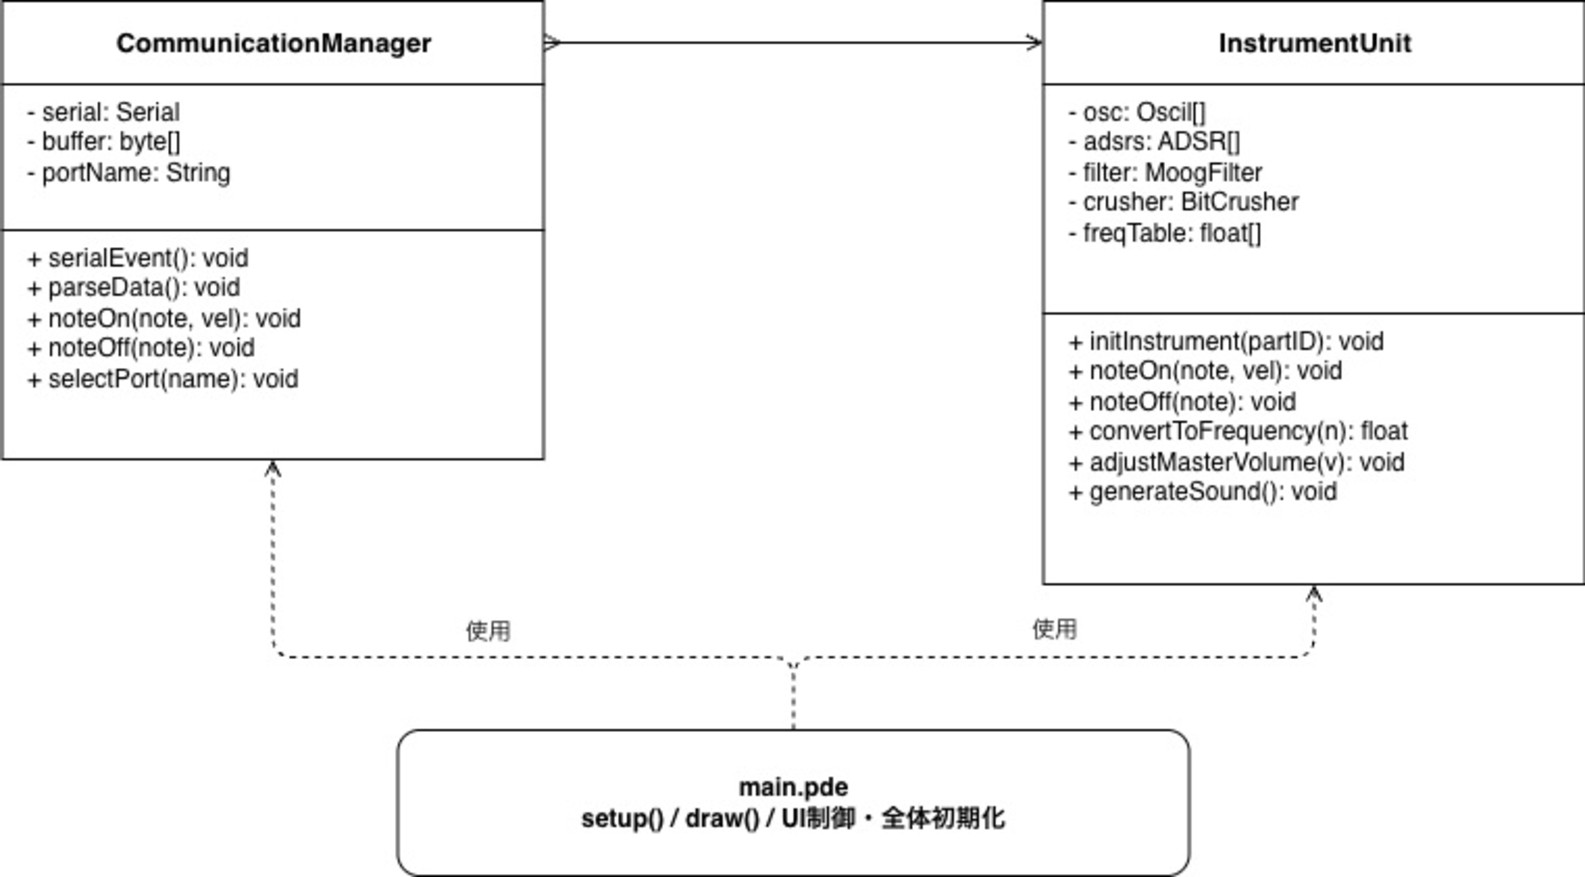
\includegraphics[width=0.85\linewidth]{figures/tantoD/class_diagram_D.pdf}
  \caption{クラス図（CommunicationManager / InstrumentUnit / main.pde）}
  \label{fig:class_D}
\end{figure}

本システムは以下の主要クラスで構成される．

\begin{itemize}

  \item \texttt{CommunicationManager} \\
  シリアル通信の受信および4バイトパケット（NOTE\_OFF / NOTE / VEL / LONG）の
  パースを行い，前音消音および新規発音イベントをInstrumentUnitへ通知する．
  パート種別は各PCのシリアル接続で確定するため，NOTEバイトはすべて
  音名インデックス（0〜5または6）として解釈する．

  \item \texttt{InstrumentUnit} \\
  受信イベントに基づき，音高変換，楽器選択，
  およびUGenチェーンによる音響生成処理を統括する．
  発音ごとにボイス（楽器インスタンス）を生成してリスト（\texttt{activeVoices}）で管理し，
  NOTE\_OFFフラグ=0の場合は前音を残したまま新規ボイスを重ね，
  NOTE\_OFFフラグ=1の場合はボイスをReleaseへ移行させてリストから除去することで
  多重発音を実現する．

\end{itemize}

音名インデックスからの周波数変換は，
平均律式 $f = 440 \times 2^{(n-69)/12}$\,[Hz] を用いる．
インデックスとMIDIノート番号の対応を表\,\ref{tab:midi_table}に示す．

\begin{table}[H]
  \centering
  \caption{音名インデックス → MIDIノート番号 → 周波数 変換テーブル}
  \label{tab:midi_table}
  \begin{tabular}{cccc}
    \hline
    インデックス（担当C） & 音名 & MIDIノート番号 $n$ & 周波数 $f$\,[Hz] \\
    \hline
    0   & C4（ド） & 60              & 261.63 \\
    1   & D4（レ） & 62              & 293.66 \\
    2   & E4（ミ） & 64              & 329.63 \\
    3   & F4（ファ）& 65             & 349.23 \\
    4   & G4（ソ） & 67              & 392.00 \\
    5   & A4（ラ） & 69（基準）      & 440.00（基準） \\
    \hline
    6   & 休符     & —               & 発音なし \\
    \hline
  \end{tabular}
\end{table}

Velocityは0〜127の値をADSRのSustainレベル（0.0〜1.0）へ正規化し，
音量制御に反映する．
LONGバイトは音価（\texttt{2}=2分音符 / \texttt{4}=4分音符 / \texttt{8}=8分音符）を示し，
新規発音時にADSRの減衰（Decay）およびリリース（Release）時間へ倍率として反映することで，
響き・余韻の長さを調整する（2分音符は長め，4分音符は標準，8分音符は短め）．
発音中の音を実際に停止するタイミングはLONGではなくNOTE\_OFF=1の受信で制御する．

NOTE\_OFFフラグ=1のパケット受信時には前音ボイスの\texttt{noteOff()}を呼び出し，
続くNOTEバイトが休符（6）でなければ新規ボイスを生成して\texttt{noteOn()}で発音を開始する．
フェルマータ中は担当Cが次パケットの送信を保留するため，
Sustainが自動的に延長される．
NOTE\_OFFフラグ=0の場合は前音を消音せずに新規発音を重ねることで多重発音を実現する．

\subsubsection{関数設計}

主要な関数を以下に示す．

\begin{itemize}

  \item \texttt{setup()} \\
  Minim，AudioOutput，およびシリアル通信の初期化を行う．
  各楽器パートのInstrumentUnitインスタンスを生成し，
  UGenチェーンをAudioOutputへ接続する．

  \item \texttt{draw()} \\
  メインループとして動作し，
  UIコンポーネント（受信データモニタ・マスターボリューム）の描画更新を行う．

  \item \texttt{serialEvent()} \\
  シリアルデータ受信時に自動的に呼び出され，
  受信バイトをバッファへ格納する．

  \item \texttt{parseData()} \\
  受信バッファから4バイト単位でデータを取り出し，
  NOTE\_OFF（\texttt{1}=前音停止 / \texttt{0}=継続），
  音名インデックス，Velocity，LONG（音価）を抽出して
  前音消音および新規発音イベントに変換する．
  NOTEバイトはすべて音名インデックス（0〜5または6）として解釈し，
  パートIDの抽出は行わない．

  \item \texttt{noteOn(int noteIndex, int velocity, int noteLength)} \\
  音名インデックスを周波数に変換し，
  新規ボイス（楽器インスタンス）を生成して\texttt{activeVoices}へ追加し，
  そのボイスの\texttt{noteOn()}でアタックを開始する．
  Velocityを正規化して振幅に反映し，
  noteLength（音価）に応じてADSRの減衰・リリース時間に倍率を乗じ，響きの長さを調整する．
  なお消音は本関数では行わず，NOTE\_OFF=1受信時の\texttt{noteOff()}で制御する．

  \item \texttt{noteOff(int noteIndex)} \\
  該当する音名インデックスのボイスを\texttt{activeVoices}から検索し，
  \texttt{noteOff()}でReleaseへ移行させたうえでリストから除去する．

  \item \texttt{convertToFrequency(int noteIndex)} \\
  音名インデックスをMIDIノート番号へ変換し，
  $f = 440 \times 2^{(n-69)/12}$\,[Hz] により周波数を算出する．

  \item \texttt{InstrumentUnit(AudioOutput out)}（コンストラクタ） \\
  各PCは担当楽器専用のスケッチを実行するため，パートIDによる選択は行わない．
  コンストラクタで当該楽器のUGenチェーン（Oscil・ADSR・Filter・BitCrusher）を構築し，\texttt{out}へ接続する．
  楽器ごとのADSRパラメータおよびフィルタ設定を適用する．
  ただしシンバルのみ，音源をOscilではなく\texttt{Sampler}（事前生成したモーダル波形）とし，
  同様に\texttt{out}へ接続する（接続構造は他楽器と共通）．

  \item \texttt{adjustMasterVolume(float value)} \\
  UIスライダーからの入力（0.0〜1.0）をデシベルに変換し，
  \texttt{out.setGain()}を呼び出して出力音量を調整する．

\end{itemize}

\subsection{処理フローの設計}

本システムの処理は，初期化フローと実行時フローの2つに分けて設計する．

\begin{figure}[H]
  \centering
  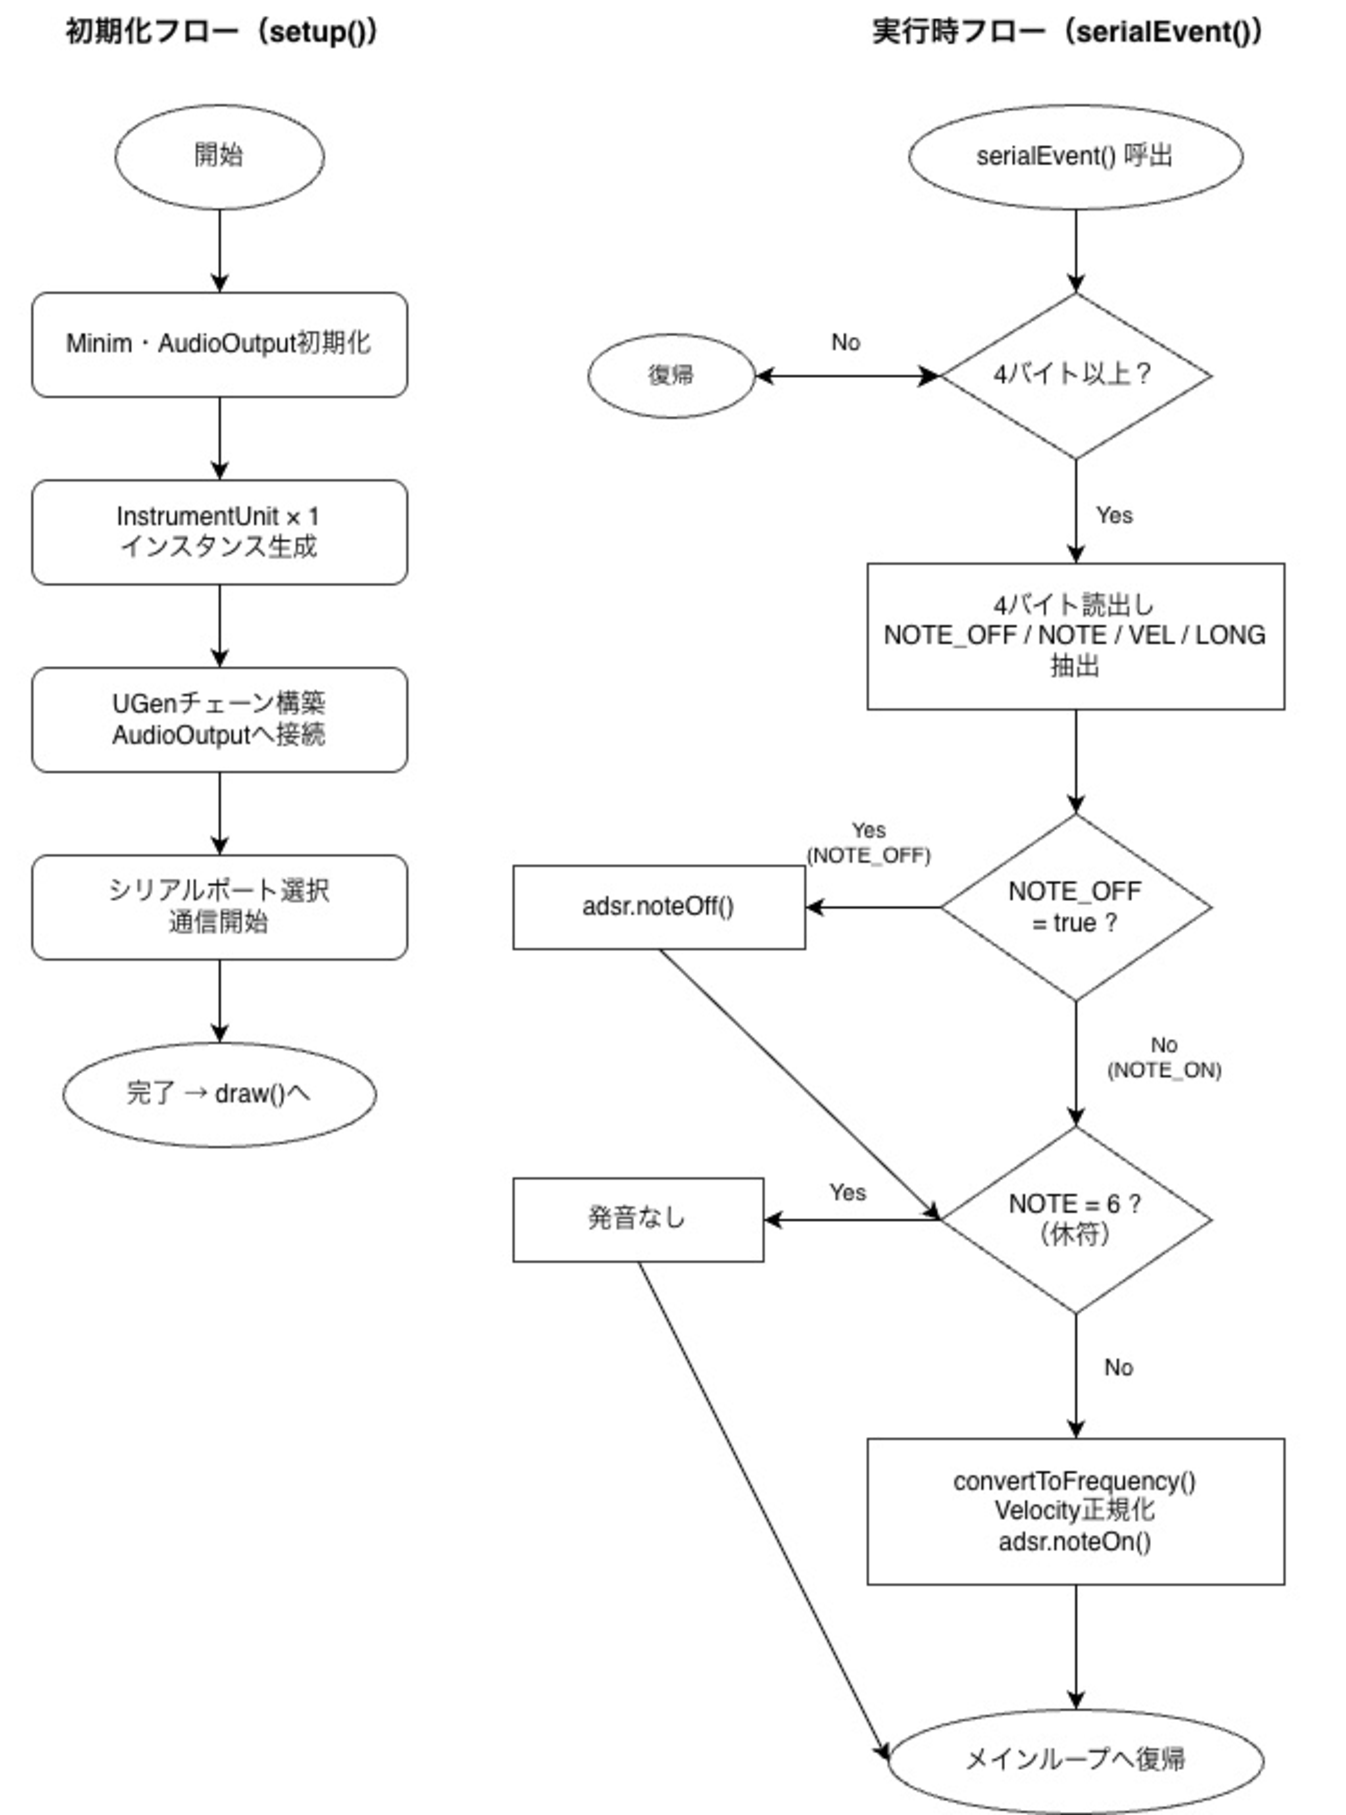
\includegraphics[width=0.85\linewidth]{figures/tantoD/process_flow_diagram_D.pdf}
  \caption{処理フロー図（初期化フロー・実行時フロー）}
  \label{fig:process_flow_D}
\end{figure}

\subsubsection*{初期化フロー（\texttt{setup()}）}

\begin{enumerate}
  \item Minimおよびシリアル通信を初期化する
  \item 担当パートに対応するInstrumentUnit（1インスタンス）を生成する
  \item UGenチェーンを構築し，AudioOutputへ接続する
  \item シリアルポートへ自動接続し，通信を開始する
\end{enumerate}

\subsubsection*{実行時フロー（\texttt{serialEvent()} → \texttt{parseData()}）}

\begin{enumerate}
  \item シリアルバッファに4バイト以上蓄積されているか確認する
  \item 4バイトを読み出し，NOTE\_OFF・音名インデックス・Velocity・LONGを抽出する
  \item NOTE\_OFFフラグを判定する
  \begin{itemize}
    \item NOTE\_OFF = \texttt{1}（前音停止）の場合：
    \begin{enumerate}
      \item 現在発音中のボイスを\texttt{noteOff()}し，
            Releaseフェーズへ移行させてリストから除去する
    \end{enumerate}
    \item NOTE\_OFF = \texttt{0}（継続）の場合：
    \begin{enumerate}
      \item 前音の消音は行わない（多重発音）
    \end{enumerate}
  \end{itemize}
  \item 音名インデックスが6（休符）であれば新規発音せずに終了する
  \item \texttt{convertToFrequency()}で周波数を算出する
  \item Velocityを正規化して振幅に反映する
  \item LONG（音価）に応じてADSRの減衰・リリース時間に倍率を乗じ，響きの長さを設定する
  \item 新規ボイスを生成して\texttt{activeVoices}へ追加し，\texttt{noteOn()}でアタックを開始する
  \item メインループへ復帰する
\end{enumerate}

フェルマータ中は担当Cが次パケットの送信を保留するため，
Processing側は追加処理なくSustain状態が自動的に延長される．
腕再開後に次パケット（NOTE\_OFF=1）を受信した時点でReleaseへ移行し，
続く音名インデックスに基づき次音の発音を開始する．


\subsection{MOE / MOP / TPM}

\subsubsection*{MOE — 有効指標}

\begin{table}[H]
  \centering
  \caption{担当D MOE一覧}
  \label{tab:moe_d}
  \begin{tabular}{llp{8cm}}
    \hline
    ID & 指標 & 説明 \\
    \hline
    MOE-D1 & 音楽的に正確な発音・消音
           & 受信したNOTE情報を正しい音高・音色・タイミングで
             発音・消音できる \\
    MOE-D2 & 楽器らしい音色の実現
           & 各楽器（ハイハット・バス・鉄琴・ピアノ・トランペット）が
             聴衆に識別できる音色を持つ \\
    \hline
  \end{tabular}
\end{table}

\subsubsection*{MOP — 性能指標}

\begin{table}[H]
  \centering
  \caption{担当D MOP一覧}
  \label{tab:mop_d}
  \begin{tabular}{llp{3.5cm}p{5cm}}
    \hline
    ID & 性能指標 & 目標値 & 測定方法 \\
    \hline
    MOP-D1 & 受信→発音遅延
           & $\leq 50$\,ms
           & C2テスト: パケット受信タイムスタンプとMinimの
             発音開始を計測（可能であればオシロ） \\
    MOP-D2 & 消音確実性
           & NOTE\_OFF=1受信後 $\leq 100$\,ms以内に確実に消音
           & C2テスト: 録音データで消音タイミングを確認 \\
    MOP-D3 & 音高精度
           & 指定音名との誤差 $\pm 5$\,cent以内
           & チューナーアプリで各音名の発音周波数を計測 \\
    MOP-D4 & Serial受信エラーなし
           & 通し演奏中に受信パースエラー 0回
           & S1テスト: エラーカウンタ変数をシリアルで監視 \\
    \hline
  \end{tabular}
\end{table}

\subsubsection*{TPM — 技術性能指標（開発中に継続監視）}

\begin{table}[H]
  \centering
  \caption{担当D TPM一覧}
  \label{tab:tpm_d}
  \begin{tabular}{lp{4cm}p{3cm}p{4.5cm}}
    \hline
    ID & 監視項目 & 監視タイミング & 判定基準 \\
    \hline
    TPM-D1 & 4バイト受信パーサの動作確認
           & 修正後・P7テスト時
           & \texttt{NOTE\_OFF=1}で前音消音，
             \texttt{0}で継続が
             正しくトリガーされること \\
    TPM-D2 & 音名インデックス→周波数変換の整合性
           & 実装着手時（C-D合意後）
           & C4=0のインデックスが
             $f=261.6$\,Hzに変換されること \\
    TPM-D3 & ADSRパラメータの音色調整状況
           & 実装中・P7テスト時
           & 各楽器が識別可能な音色を持ち，
             音量バランスが取れていること \\
    TPM-D4 & Minimライブラリ動作環境の統一
           & 実装着手前
           & 5台のPC全てでProcessing + Minimが
             正常動作すること（バージョン統一） \\
    TPM-D5 & \texttt{out.setGain()}の動作確認
           & P7テスト時
           & スライダー操作により音量が0〜100\,\%の
             範囲で連続的に変化すること \\
    \hline
  \end{tabular}
\end{table}

\subsection{テストの設計}

本システムのテストは，事前確認テスト・結合テスト・システムテストの
3フェーズで実施する．
なお，P7が事前確認テスト，C2が結合テスト，S1がシステムテストにそれぞれ対応する．
各テストの内容および合格基準を表\,\ref{tab:test_d}に示す．

\begin{table}[H]
  \centering
  \caption{担当D テスト計画}
  \label{tab:test_d}
  \begin{tabular}{llp{5cm}p{4cm}}
    \hline
    ID & テスト名 & 内容 & 合格基準 \\
    \hline
    P7 & Processing音響出力確認
       & 手動で4バイト（NOTE\_OFF=1, NOTE, VEL, LONG）を
         シリアル送信し，指定音が発音されるか確認する
       & 正しい音高・音量で発音される \\
    C2 & C-D間同期確認
       & Arduinoのパケット送信から発音までの遅延を計測する．
         またNOTE\_OFF=1受信時に確実に前音が消音されるか確認する
       & 遅延 $\leq$ 50\,ms，NOTE\_OFF=1時に確実に消音，
         発音ずれ $\leq$ 1拍 \\
    S1 & 通し演奏・BPM維持評価
       & 全15小節以上の通し演奏で音響品質・タイミングを評価する
       & BPM誤差 $\pm$5\,bpm以内，発音ミスなし \\
    \hline
  \end{tabular}
\end{table}

また，開発中の音色調整を目的として，以下の評価を随時実施する．

\begin{itemize}
  \item 音高精度確認 \\
  チューナーアプリで各音名の発音周波数を計測し，
  目標値との誤差が$\pm$5\,cent以内であることを確認する．

  \item 聴感評価 \\
  各楽器音が聴衆に識別可能な音色を持つことを
  人間の聴感により確認する．
\end{itemize}